\section{Introduction}
Recent advances in biomedical image analysis have assisted many pathologists and biologists to facilitate their researches \cite{Chen2016b, Ronneberger2015,Chen2016c,Lieman-Sifry2017,Paszke2016,Tseng2017,Sirinukunwattana2015b}.
Among these researches, a significant application is to obtain the accurate segmentation of specific membrane objects in a biomedical image, such as lumenal glands, synaptic vesicles and cells.
Especially, the morphological shape and spatial distribution of synaptic vesicles are helpful to study the neural activity in different brain regions, while morphological statistics of lumenal glands are widely used for assessment of the malignancy degree of adenocarcinomas.
%
Conventionally, these crucial steps are performed by human expert, which are time-consuming and suffer from subjective factors.
\cxj{For example, how long does it take to handle a task..?}
Therefore, it is significantly demanded to improve the efficiency as well as the reliability with automatic segmentation methods.

\begin{figure}
    \begin{center}
        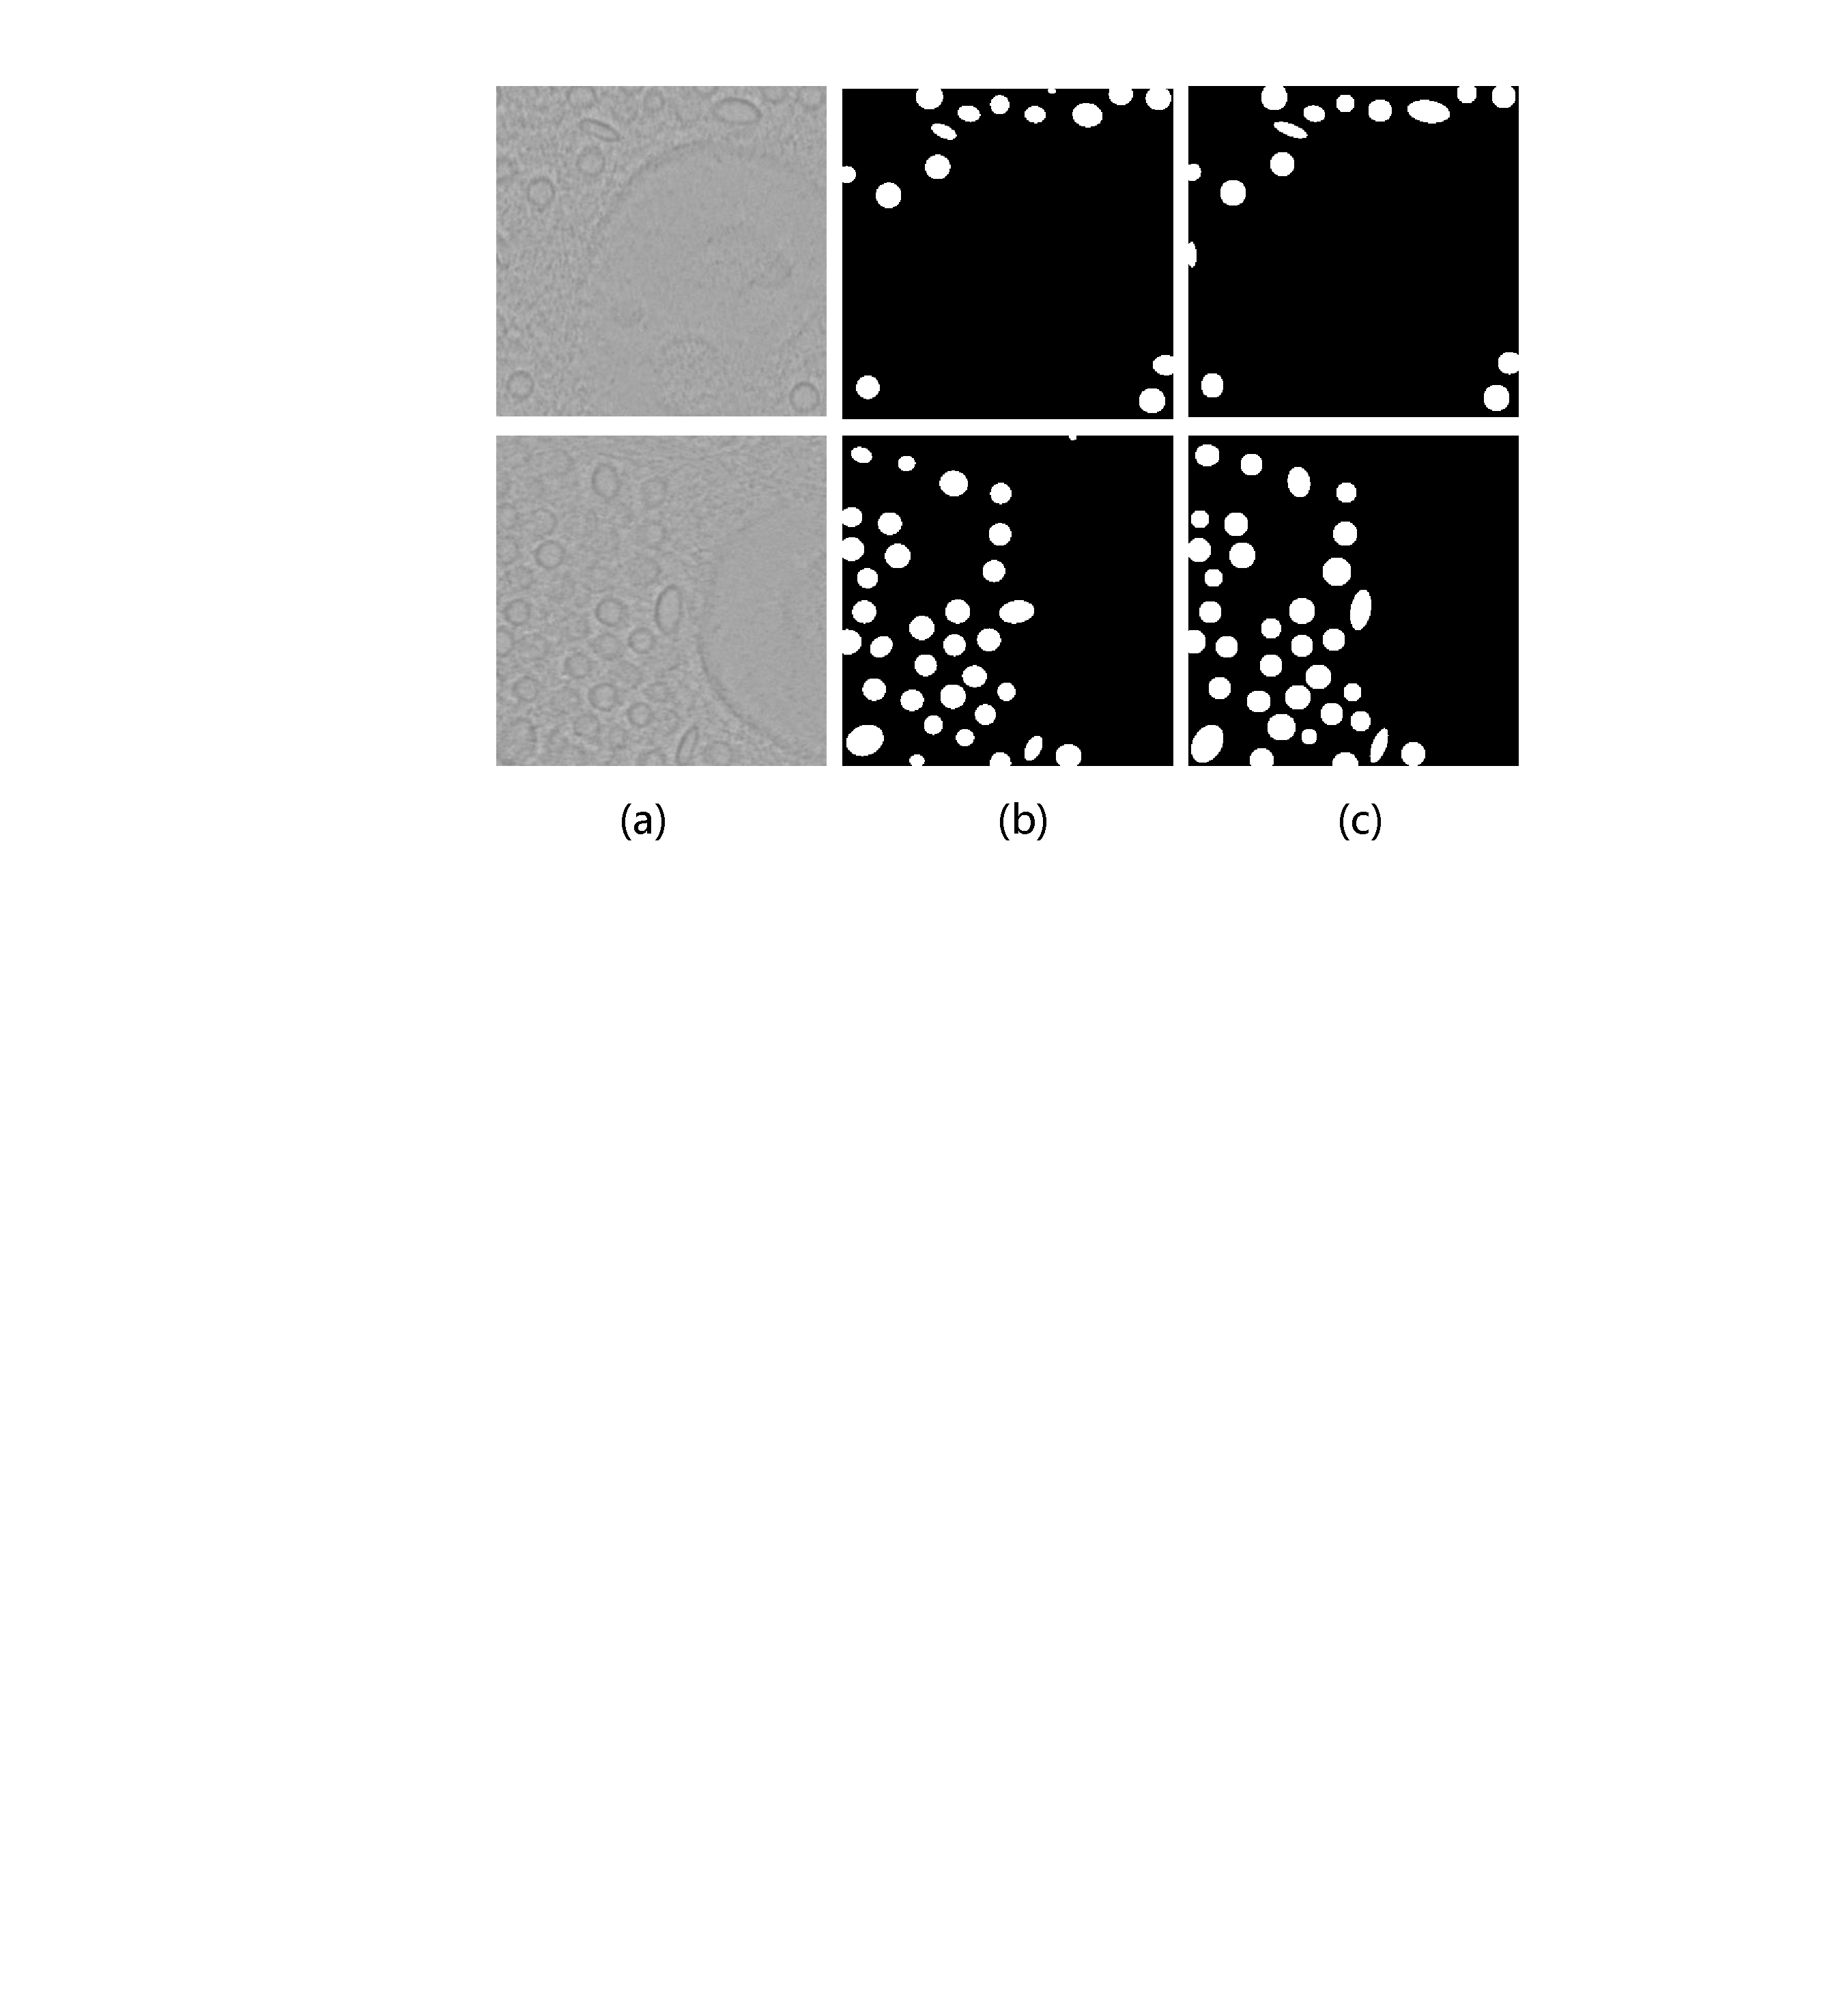
\includegraphics[width=3.3in]{figures/FigImg.pdf}
    \end{center}
    \caption{An example showing the challenges of biomedical segmentation: (a) synaptic vesicle image; (b) results from proposed SCNN by incorporating prior shape knowledge; (c) annotations by experts.}
    \label{FigImgs}
\end{figure}

However, it is non-trivial to automatically segment biomedical images.
First, biomedical images are usually noisy and obscure caused by deficient imaging techniques, as shown in Figure~\ref{FigImgs} (a).
Second, most membrane objects in biomedical images are arranged compactly and densely arrangement, thus it is hard to separate objects individually, which is known as the touching problem.
Third, in some pathological cases, the inter-class deformation of some pathological objects are much different, while the shape of most healthy objects are regular.
It is hard to incorporate prior shape knowledge to optimize most regular objects without restricting the model generalization to pathological cases \cite{Sirinukunwattana2015b}.

Recently, deep neural networks have demonstrated excellent performance in biomedical image segmentation with the use of fully convolutional networks \cite{Dhungel2015,Ronneberger2015,Roth2015,Chen2015,Lieman-Sifry2017,Xu2016,Chen2016b}.
However, as most of these deep networks are based on fully convolutional networks~\cite{Long2015}, the pooling and downsampling layers make them inevitable to get poorly localized object boundaries.
To increase the boundary accuracy, many efforts have been made recently. An U-shaped deep network called U-net~\cite{Ronneberger2015} is proposed for biomedical image segmentation. 
By employing the skip connections between contracting and expanding paths, context information can be directly propagated to higher resolution layers for detail preserving.
Several improvements of U-net were proposed soon afterwards.
DeepVentricle~\cite{Lieman-Sifry2017}, which uses the same padding instead of valid padding, has been successfully used for cardiac segmentation.
Recently, DCAN~\cite{Chen2016a} integrates complementary information of objects and contours in a multi-task learning framework to separate the clustered objects into individual ones.\cxj{for more accurate boundaries?}
Although these methods achieved promising results in their segmentation tasks, they may fail to achieving satisfying performance in denser and smaller objects with regular shapes, such as synaptic vesicle dataset shown in Figure~\ref{FigImgs}.

In this paper, we propose a first Shape-Constrained neural network (SCNN) to segment dense objects by inherently incorporating prior shape knowledge into network.
Similar with \cite{Chen2016a}, we formulate the network as a multi-task learning framework by simultaneously predicting an objectness scores map and an auxiliary map for an input image.
Instead of contour probability \cite{Chen2016a,Chen2016,Bertasius2016}, our SCNN learns the parameterized expression of objects shape, which emphasizes more on the overall shape of objects.
Inspired by Region Proposal Networks in \cite{Ren2015}, our SCNN simultaneously predicts objectness scores and a set of shape parameters, which formulate the shape of a nearest object, at each position.
The complementary information in auxiliary parameters can not only separate objects into individual ones, but also optimize their shapes.

However since the objects are not always regular, their shape cannot be parameterized uniformly and constrained strictly.
Therefore, we select a best representative shape as constraint and adopt a local optimizing strategy in fusion step to find a balance between regularization and unconstraint.
In this way, our SCNN not only optimizes the segmentation of regular objects with prior shape knowledge, but also well accommodates serious deformable objects.
\cxj{what do you mean here?}

Furthermore, predicting the shape parameters of objects accurately is a significantly challenge task, because complex information is required to analyze the overall context of a neighbouring object
\cxj{Why this is more difficult? what is the challenge?}
To this end, we proposed a novel joint max pooling to improve the performance of both objectness scores and shape parameters in final fusion step by exploring the intrinsic correlation between them.
Moverover, JMP is designed as a trainable layer, which can be trained end-to-end and easily extended to any multi-task networks.

\begin{figure}
    \begin{center}
        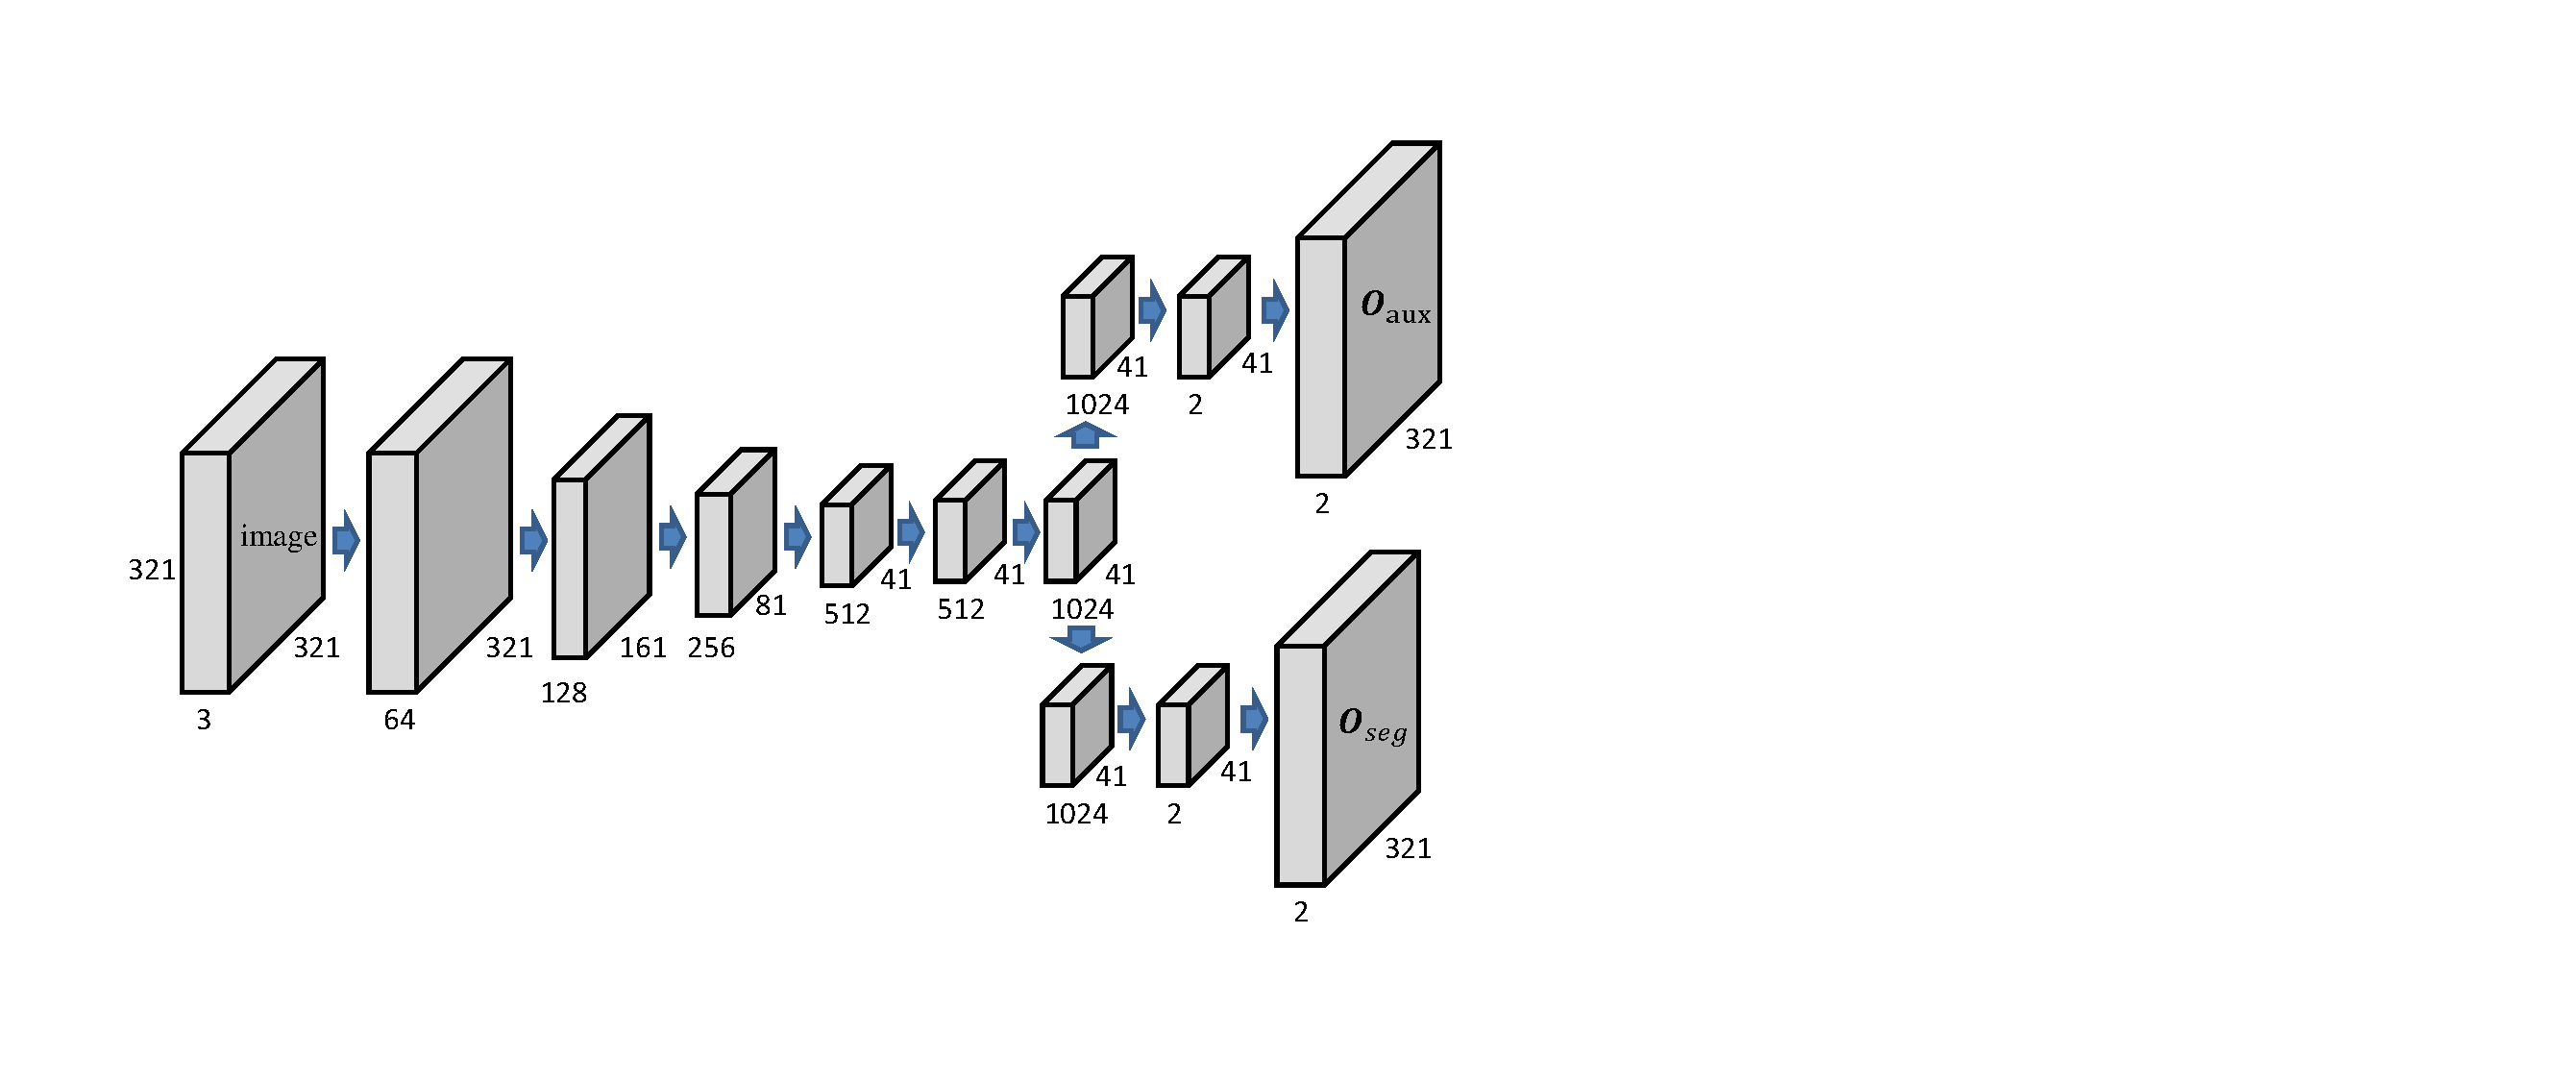
\includegraphics[width=3.3in]{figures/FigMTN.pdf}
    \end{center}
    \caption{Architecture of multi-task neural network based on FCN. \cxj{I would sugest using real images as input and output.}}
    \label{FigMTN}
\end{figure}
Overall, the contribution of this paper is three-fold:
\begin{enumerate}
	\item We first effectively incorporate shape constraint into deep neural networks.
	% for biomedical image segmentation.
	\item We propose a novel joint max pooling for benefiting both multi-task outputs.
	\item Our framework is applicable to a series of different tasks such as biomedical image segmentation, scent detection task and achieves the state-of-the-art performance.
\end{enumerate}